
\section{Resultados}

Las estrategias de control implementadas fueron probadas con dos casos de prueba: bajo una referencia estática en un punto arbitrario y bajo el seguimiento de una trayectoria circular.

El caso bajo una referencia estática se evaluó el tiempo de estabilización y el error en estado estable y en el caso de seguimiento de trayectorias se evaluó qué tan robusto es el sistema y el comportamiento del mismo fuera del punto de linealización.

La trayectoria generada a seguir por la plataforma esta definida por las siguientes ecuaciones:

\begin{equation} \label{equ: pos_tray}
    P = \begin{bmatrix}
    0.1 \cos (\omega t) \\
    0.1 \sen (\omega t) \\
    1.5
    \end{bmatrix}
\end{equation}

\begin{equation}\label{equ: vel_tray}
    \dot{P} = \begin{bmatrix}
    -0.1 \omega \sen (\omega t) \\
    0.1 \omega \cos (\omega t) \\
    0
    \end{bmatrix}
\end{equation}

Se contempla utilizar que la plataforma de la vuelta completa en 10 segundos, por lo tanto se tiene $\omega = \pi / 10$. En la simulación de la trayectoria no se contemplan movimientos en los ángulos de alabeo, cabeceo y guiñada.\\

Los controles que fueron implementados generaron diferentes resultados de la plataforma al llegar a la estabilidad. Los resultados fueron los siguientes:

\subsection{Control PD}

\begin{figure}[H]
    \centering
    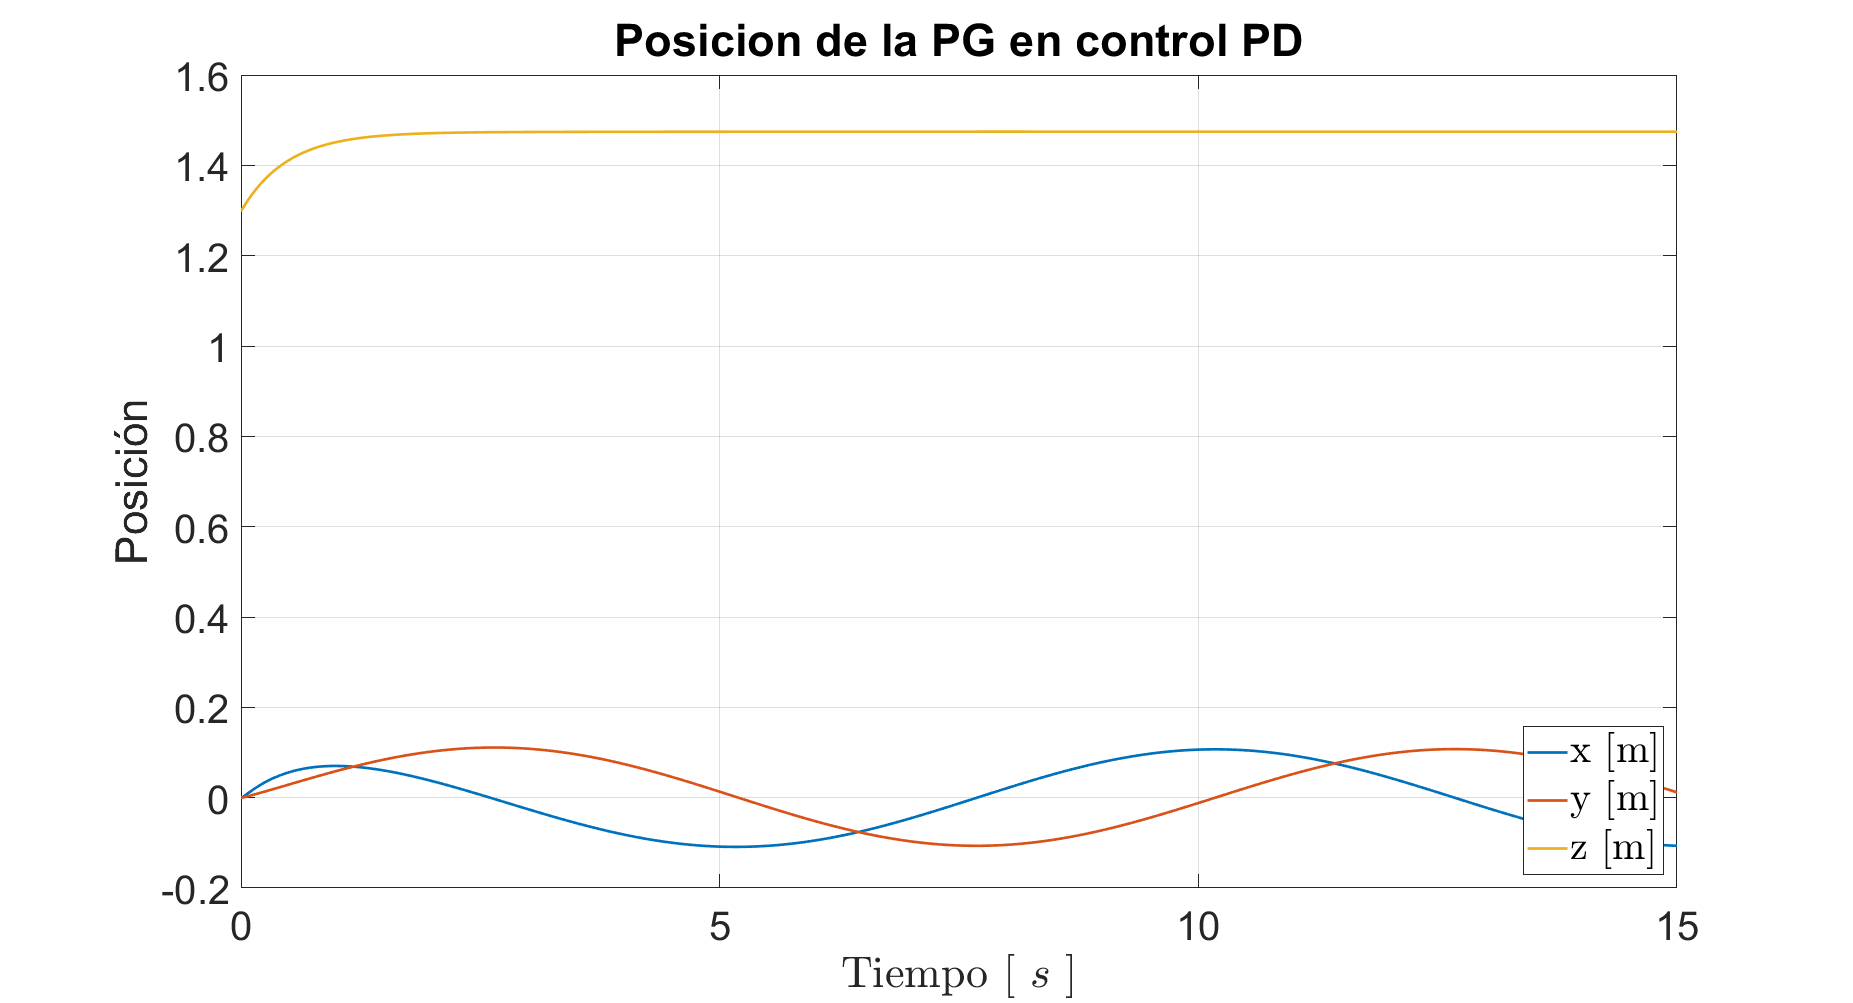
\includegraphics[width=0.4\textwidth]{posPD.png}
    \caption{Posición del sistema bajo un patrón de movimiento - PD.}
    \label{fig:PD position}
\end{figure}

\begin{figure}[H]
    \centering
    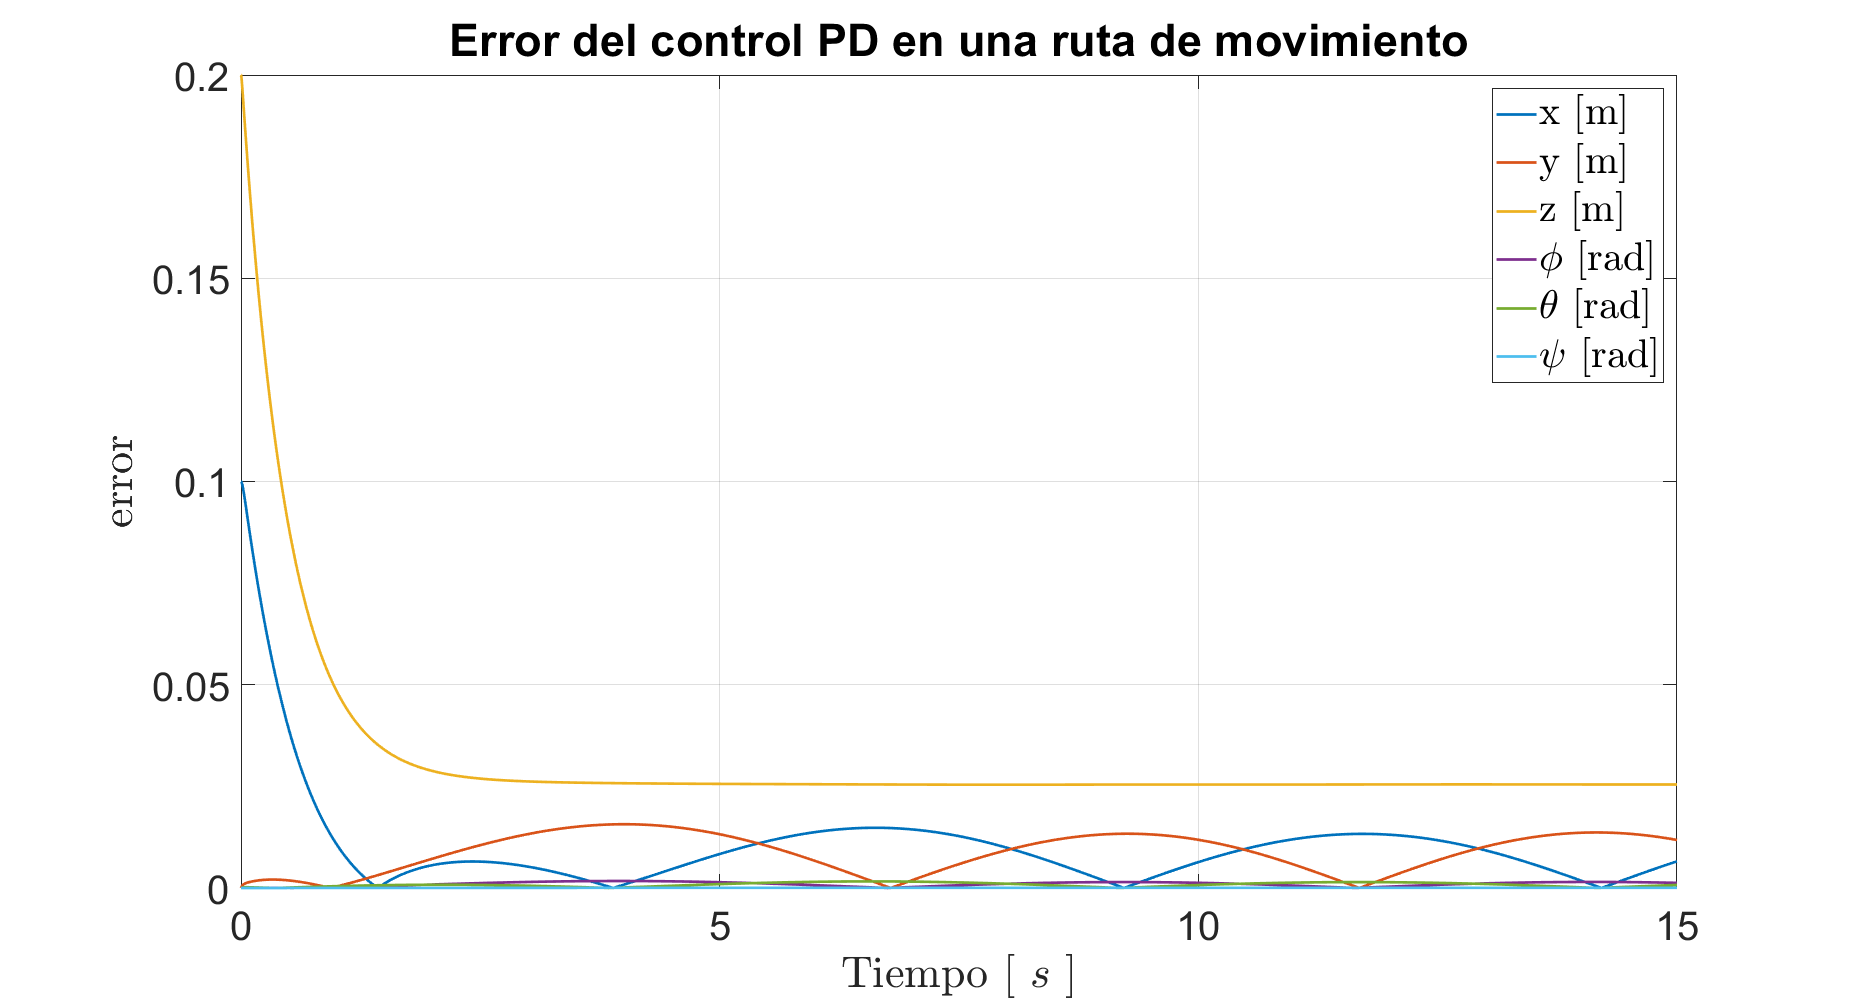
\includegraphics[width=0.4\textwidth]{errorPD.png}
    \caption{Error del sistema bajo un patrón de movimiento- PD.}
    \label{fig:PD error}
\end{figure}


\begin{figure}[H]
    \centering
    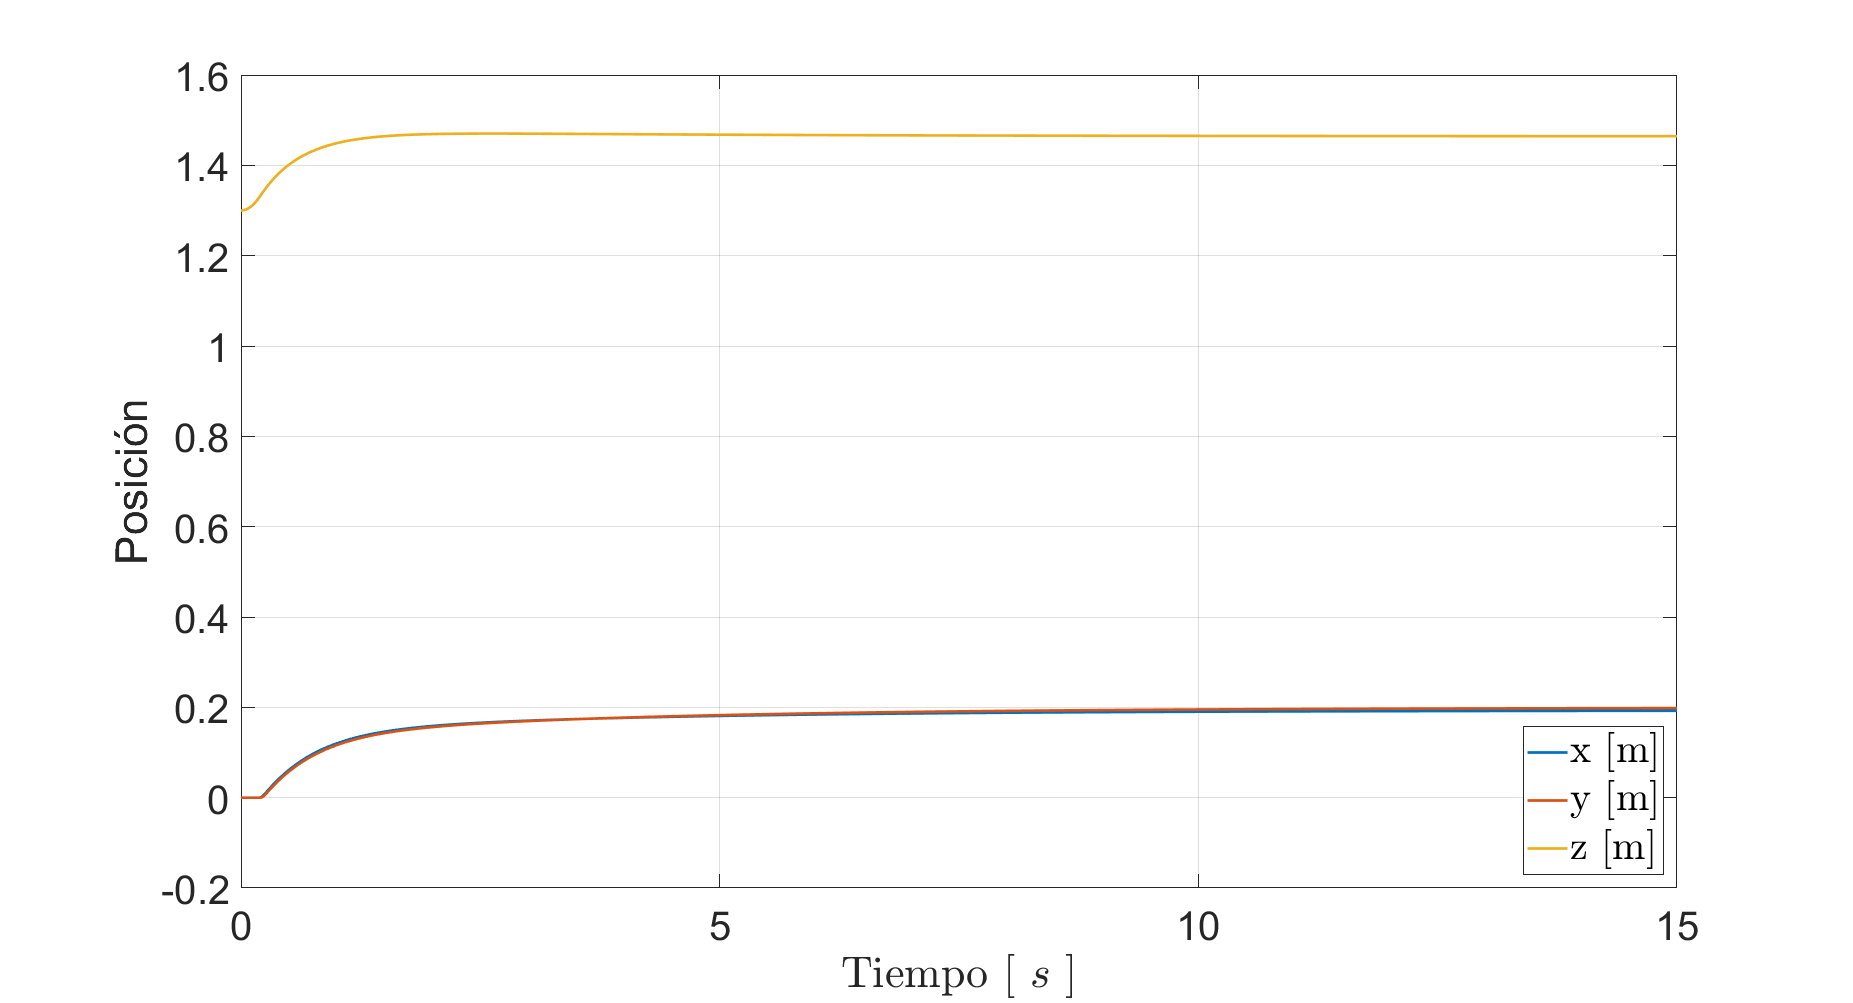
\includegraphics[width=0.4\textwidth]{posPDe.png}
    \caption{Posición del sistema bajo una referencia estática- PD.}
    \label{fig:PD positione}
\end{figure}

\begin{figure}[H]
    \centering
    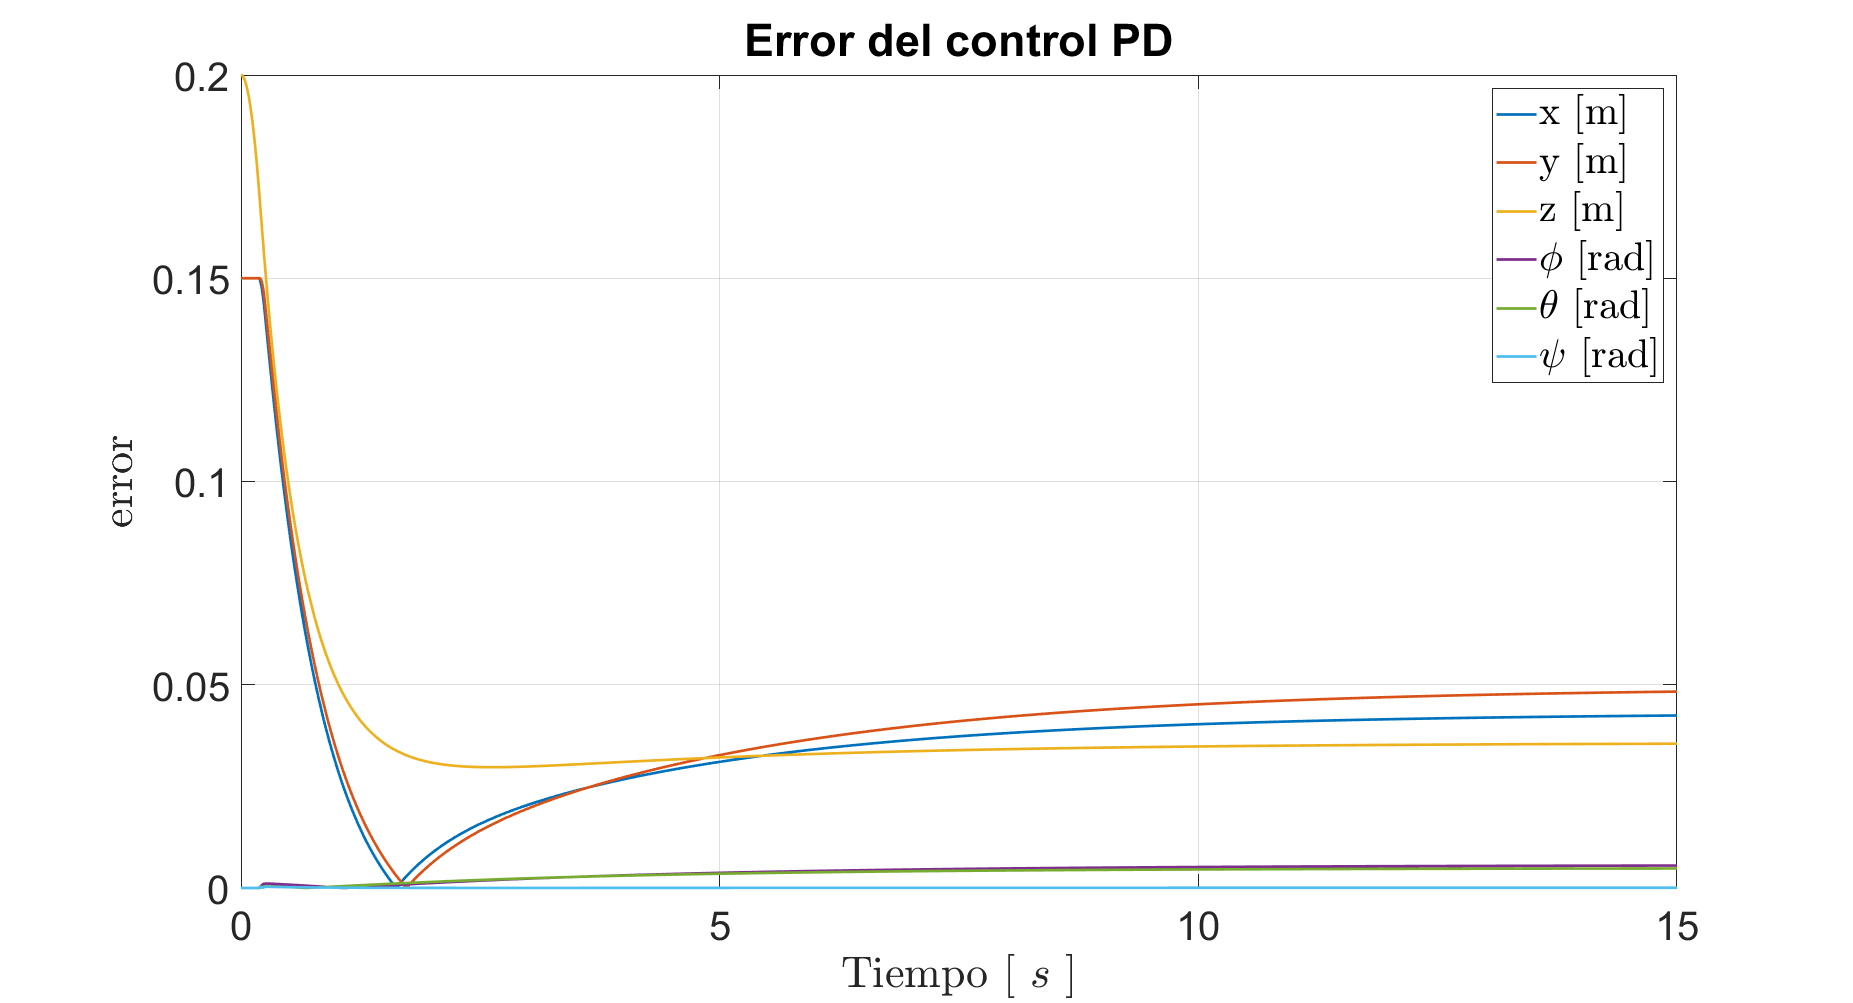
\includegraphics[width=0.4\textwidth]{errorPDe.png}
    \caption{Error del sistema bajo una referencia estática - PD.}
    \label{fig:PD errore}
\end{figure}

En las figuras \ref{fig:PD position} y \ref{fig:PD error} se observa el comportamiento de la plataforma bajo control PD para una trayectoria de movimiento generada por las ecuaciones \ref{equ: pos_tray} y \ref{equ: vel_tray}. Observando la figura \ref{fig:PD error} se visualiza que existe un error que permanece a pesar que la plataforma sigue los puntos de la trayectoria generada.

En las figuras \ref{fig:PD positione} y \ref{fig:PD errore} se observa el comportamiento de la plataforma bajo control PD para una referencia estática. Observando la figura \ref{fig:PD errore}  se visualiza que existe un error constante en los ejes X, Y y Z. Este error es muy similar al error del caso anterior, puesto que el control PD no tiene manera de corregir el error en el estado estable.

\subsection{Control PD+G}

\begin{figure}[H]
    \centering
    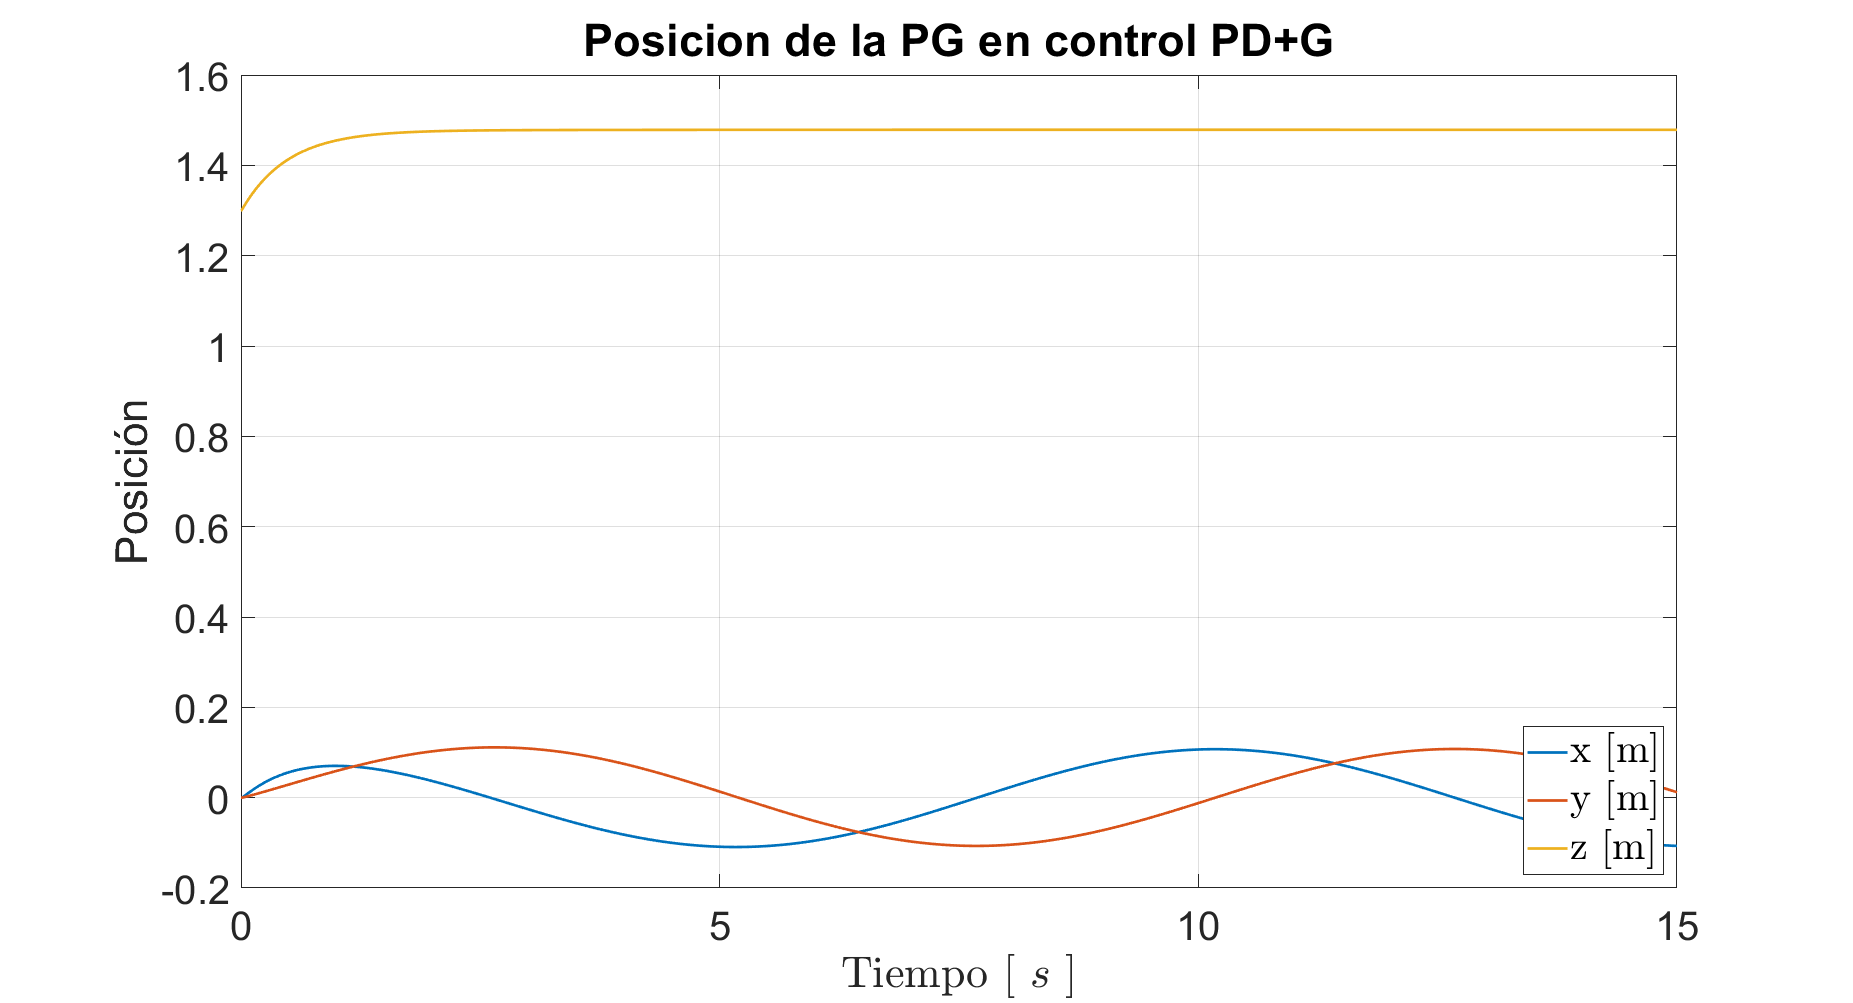
\includegraphics[width=0.4\textwidth]{posPDpG.png}
    \caption{Posición del sistema bajo un patrón de movimiento - PD+G.}
    \label{fig:PDG position}
\end{figure}

\begin{figure}[H]
    \centering
    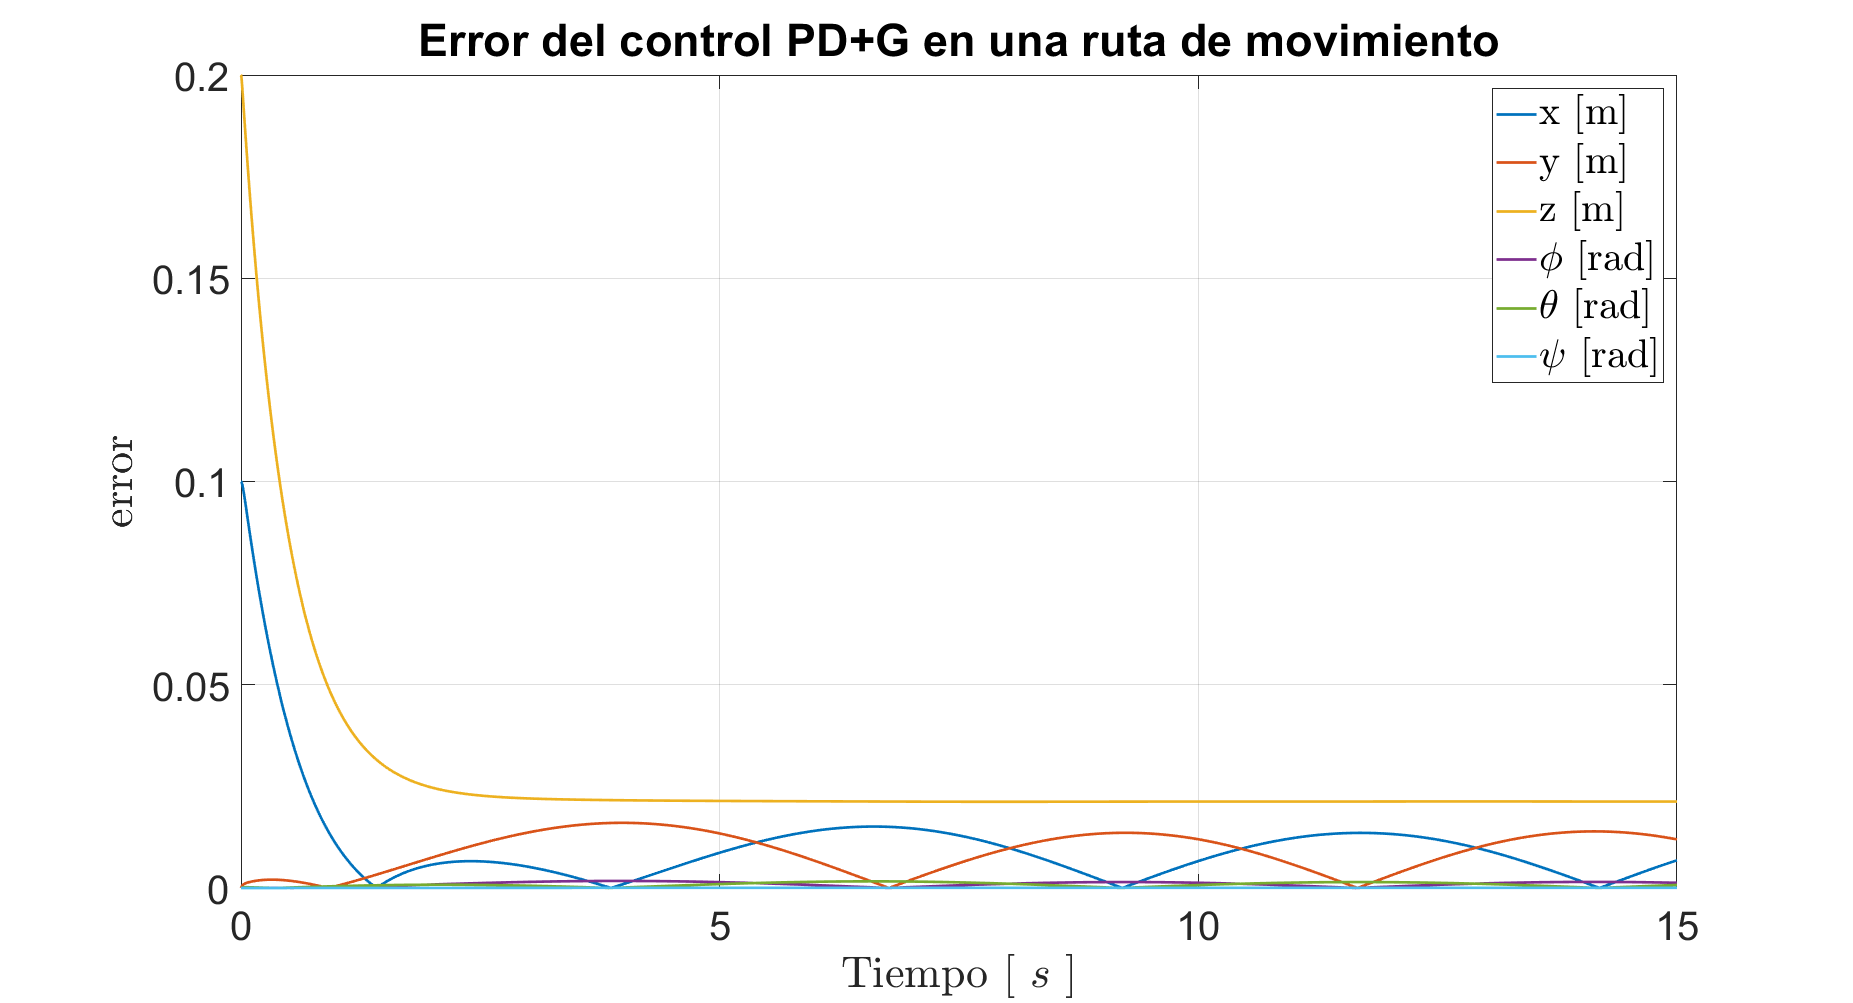
\includegraphics[width=0.4\textwidth]{errorPDpG.png}
    \caption{Error del sistema bajo un patrón de movimiento - PD+G.}
    \label{fig:PDG error}
\end{figure}

\begin{figure}[H]
    \centering
    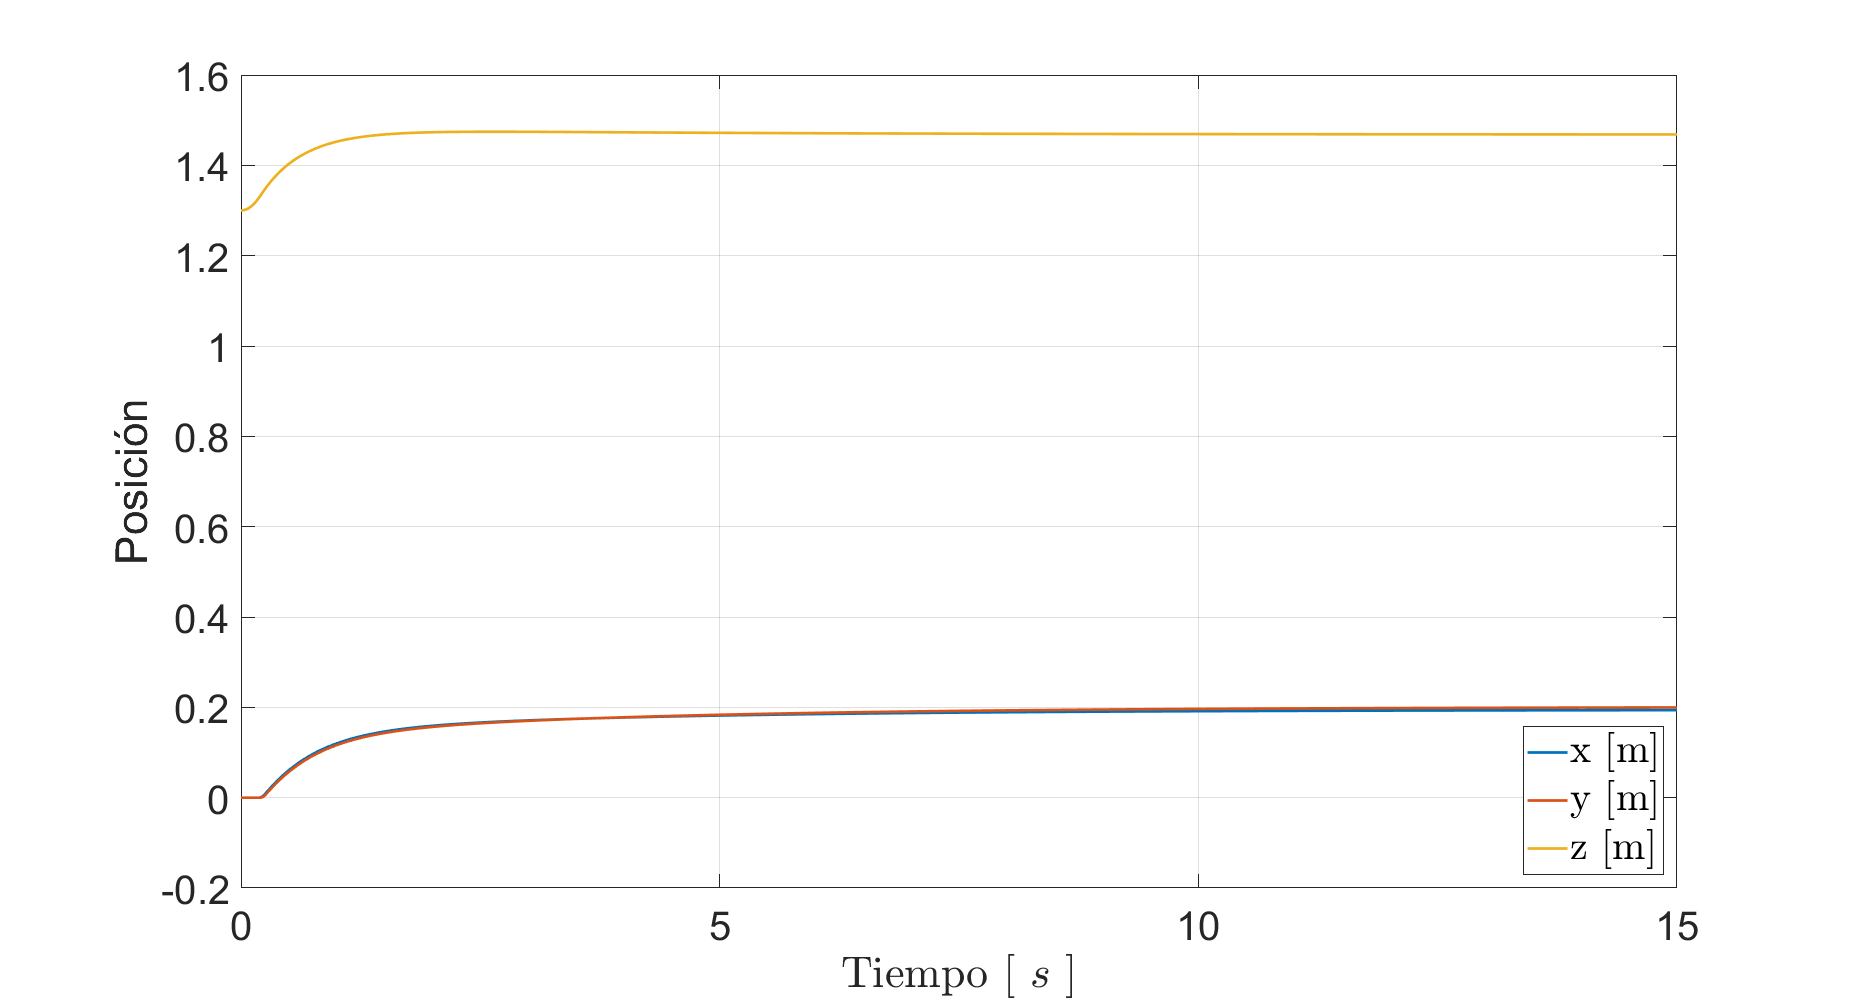
\includegraphics[width=0.4\textwidth]{posPDpGe.png}
    \caption{Posición del sistema bajo una referencia estática - PD+G.}
    \label{fig:PDG positione}
\end{figure}

\begin{figure}[H]
    \centering
    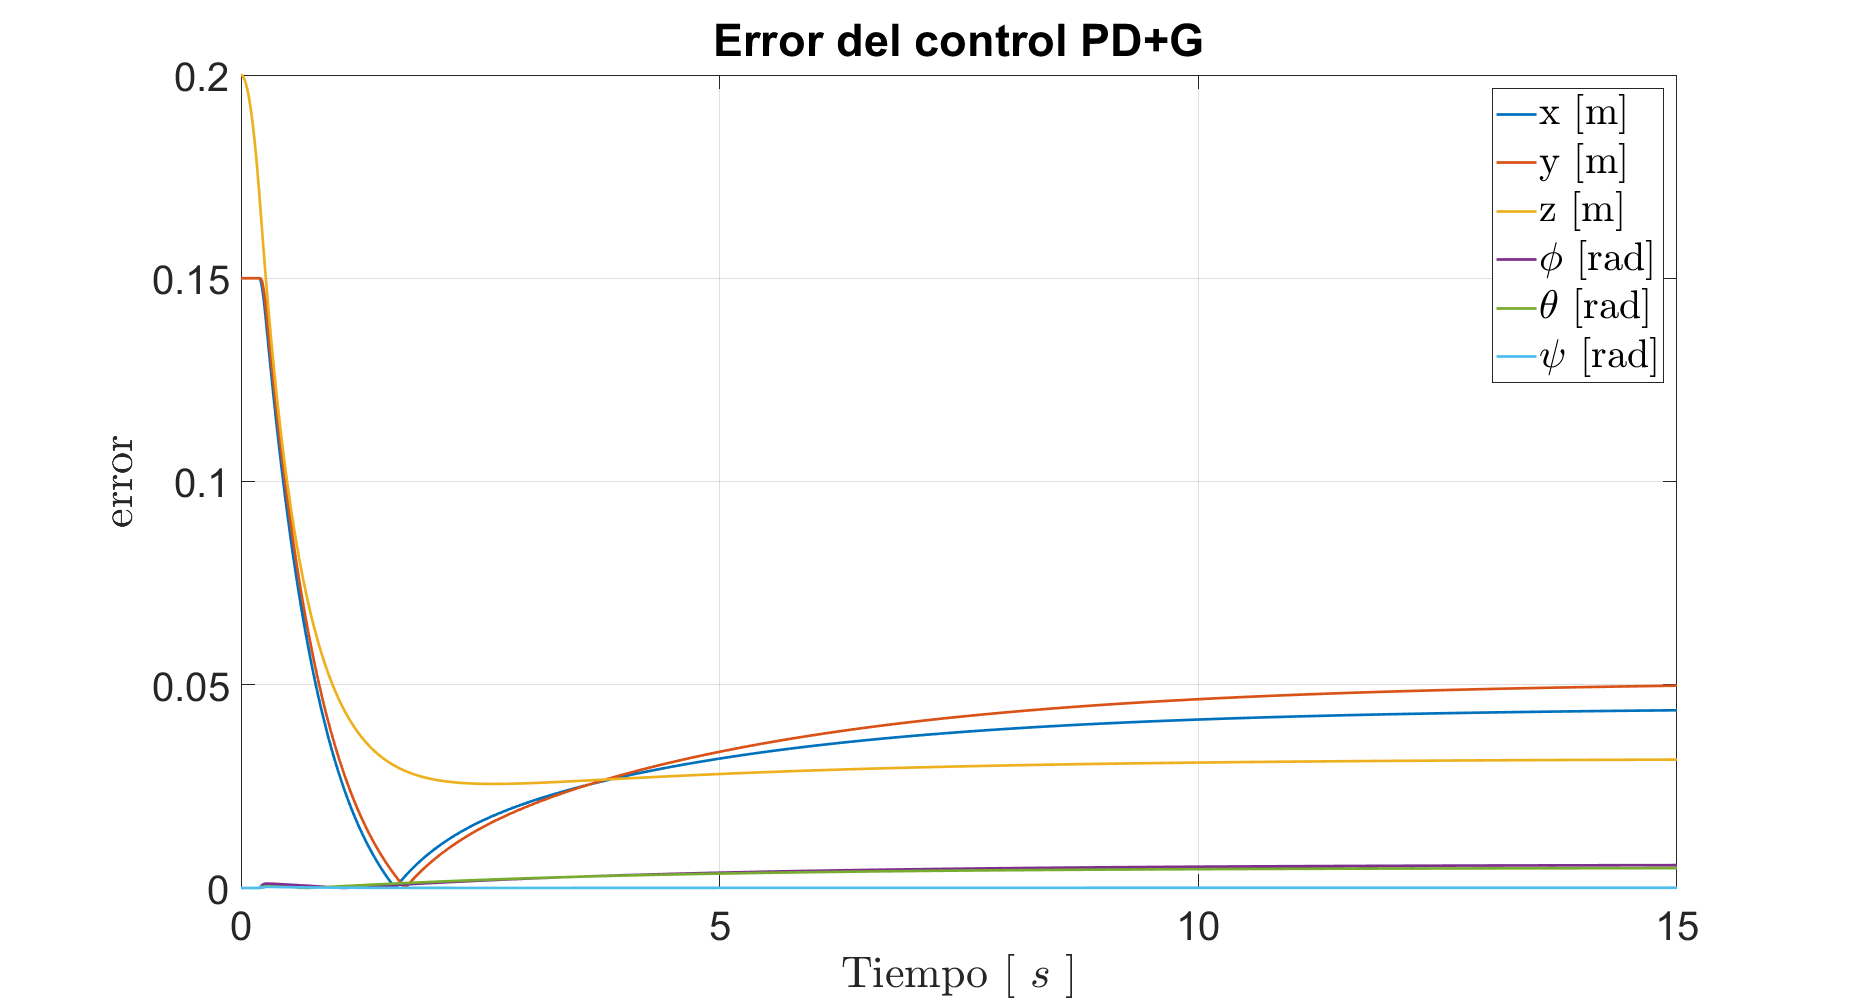
\includegraphics[width=0.4\textwidth]{errorPDpGe.png}
    \caption{Error del sistema bajo una referencia estática - PD+G.}
    \label{fig:PDG errore}
\end{figure}

En las figuras \ref{fig:PDG position} y \ref{fig:PDG error} se observa el comportamiento de la plataforma bajo control PD + G en la trayectoria de movimiento generada por las ecuaciones \ref{equ: pos_tray} y \ref{equ: vel_tray}. A diferencia del control PD, el PD + G logra compensar de mejor manera el error estacionario de la plataforma. Sin embargo debido al calculo de las ganancias del controlador en una posición específica así cuando la plataforma busca llegar a otro valor genera error debido a los términos no lineales del sistema.

En las figuras \ref{fig:PDG positione} y \ref{fig:PDG errore} se observa el comportamiento de la plataforma bajo control PD + G en una referencia estática y al igual que en el patrón de movimiento se acerca a la referencia más que en el control PD. Y por el calculo de las ganancias del controlador en una posicion específica genera error por no estar en la referencia.

\subsection{Control PID}

\begin{figure}[H]
    \centering
    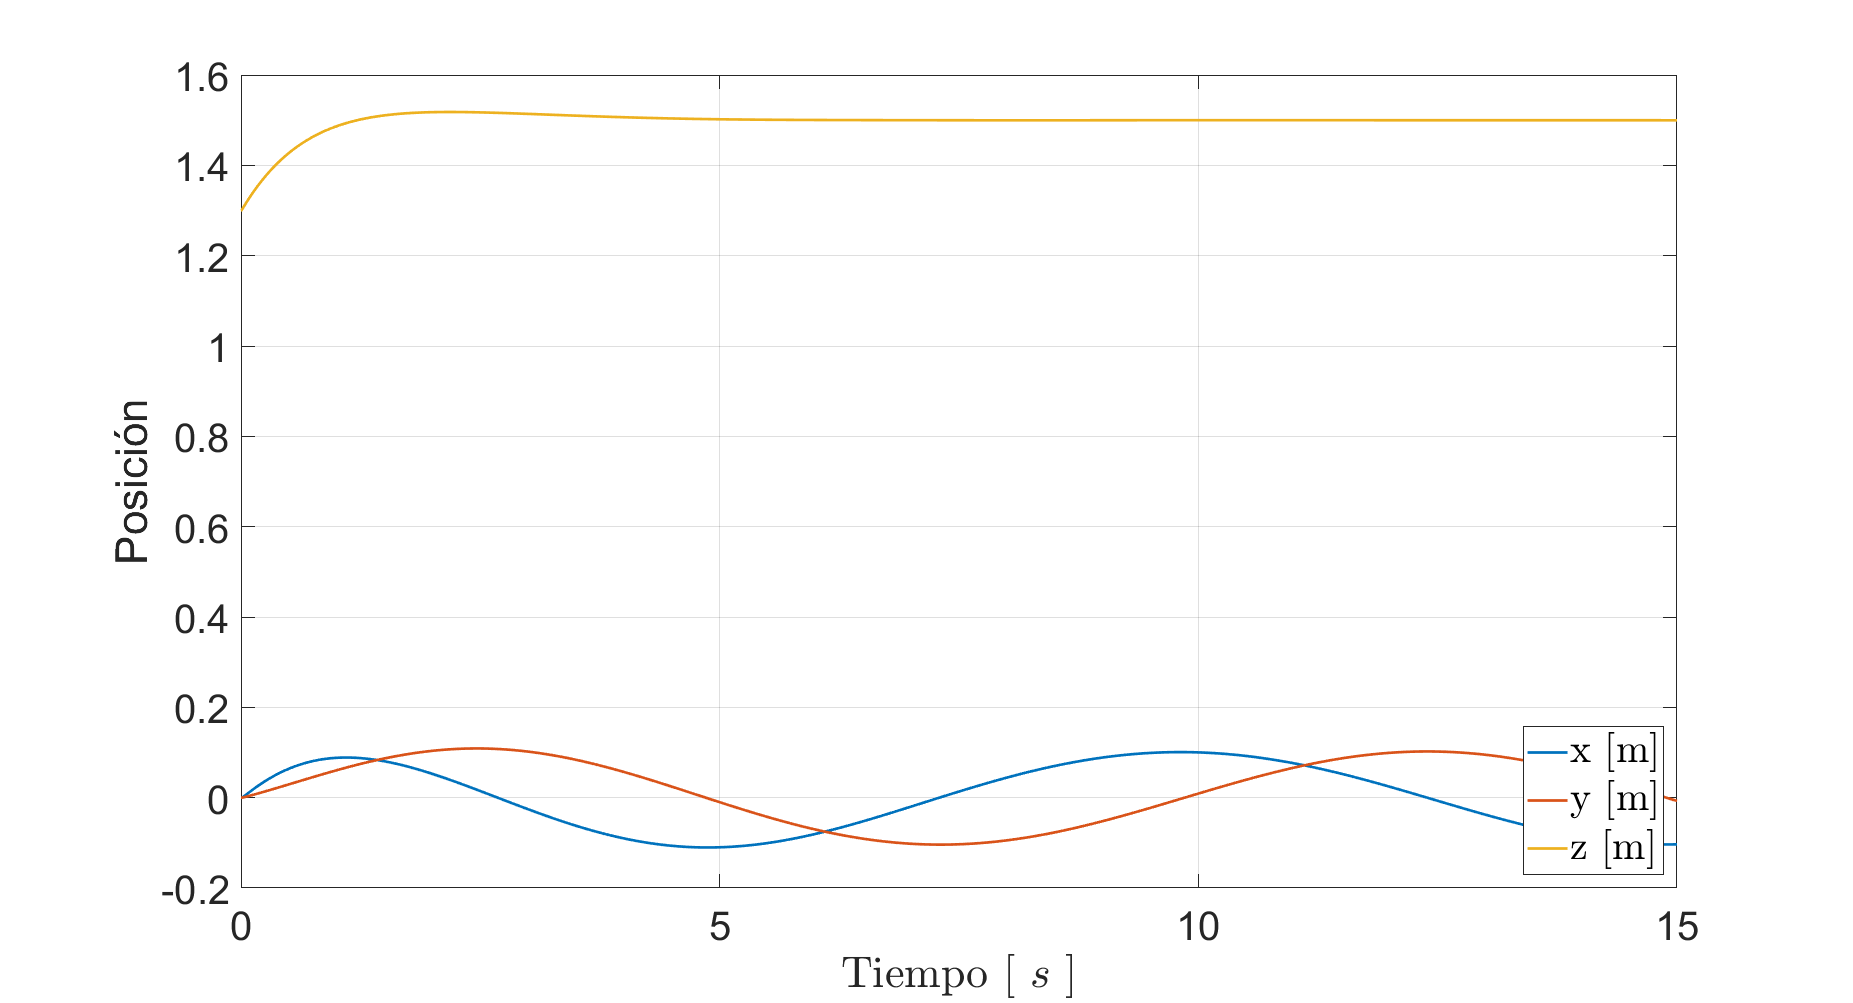
\includegraphics[width=0.4\textwidth]{posPID.png}
    \caption{Posición del sistema bajo un patrón de movimiento - PID.}
    \label{fig:PID position}
\end{figure}

\begin{figure}[H]
    \centering
    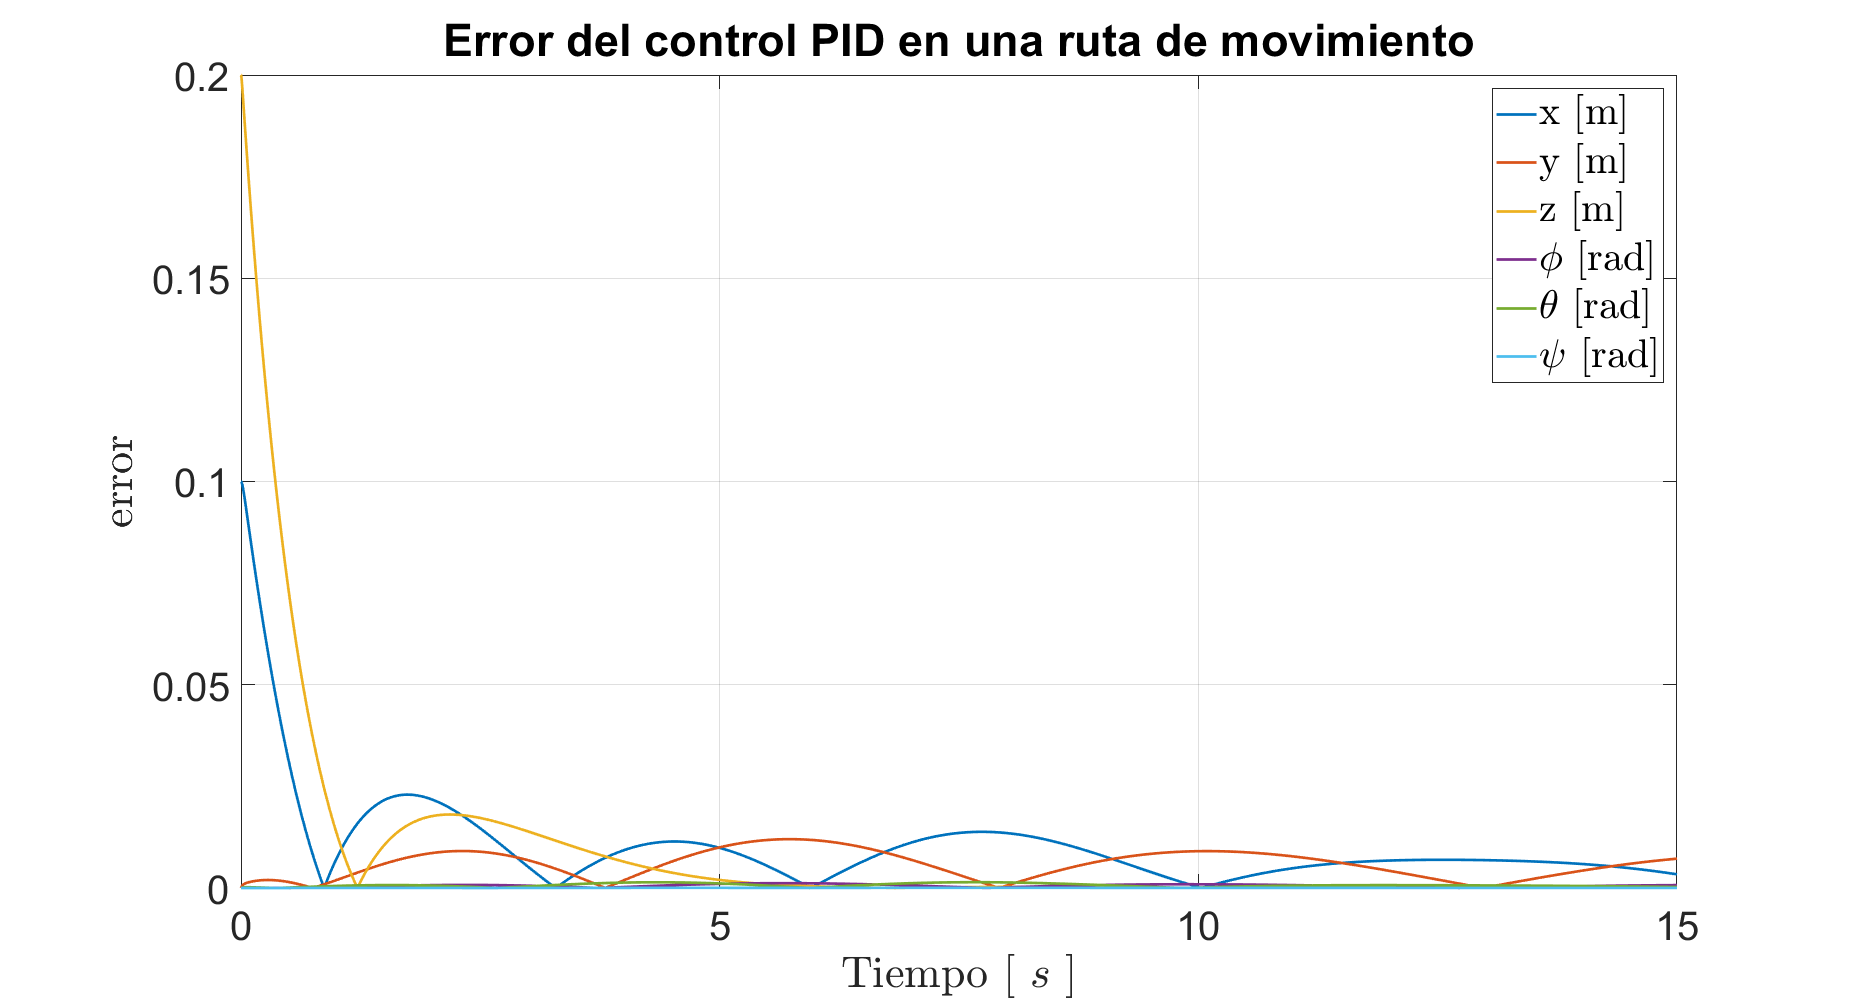
\includegraphics[width=0.4\textwidth]{errorPID.png}
    \caption{Error del sistema bajo un patrón de movimiento - PID.}
    \label{fig:PID error}
\end{figure}

\begin{figure}[H]
    \centering
    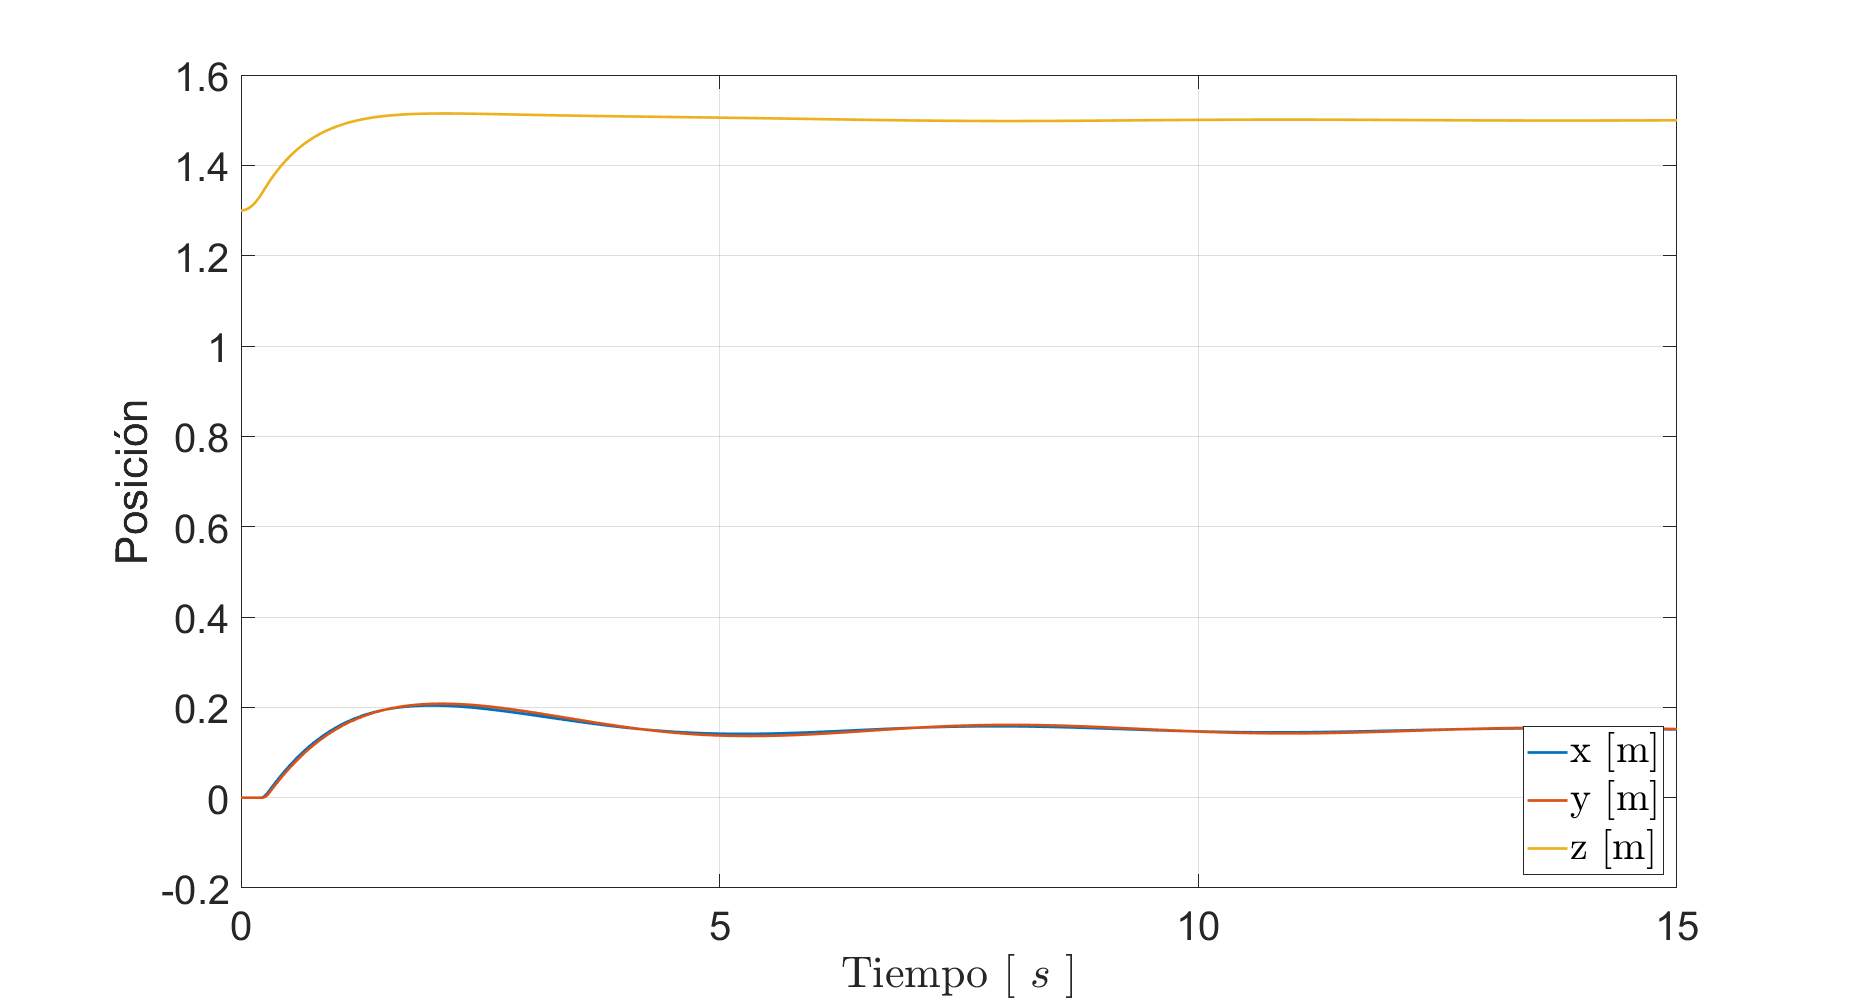
\includegraphics[width=0.4\textwidth]{posPIDe.png}
    \caption{Posición del sistema bajo una referencia estática - PID.}
    \label{fig:PID positione}
\end{figure}

\begin{figure}[H]
    \centering
    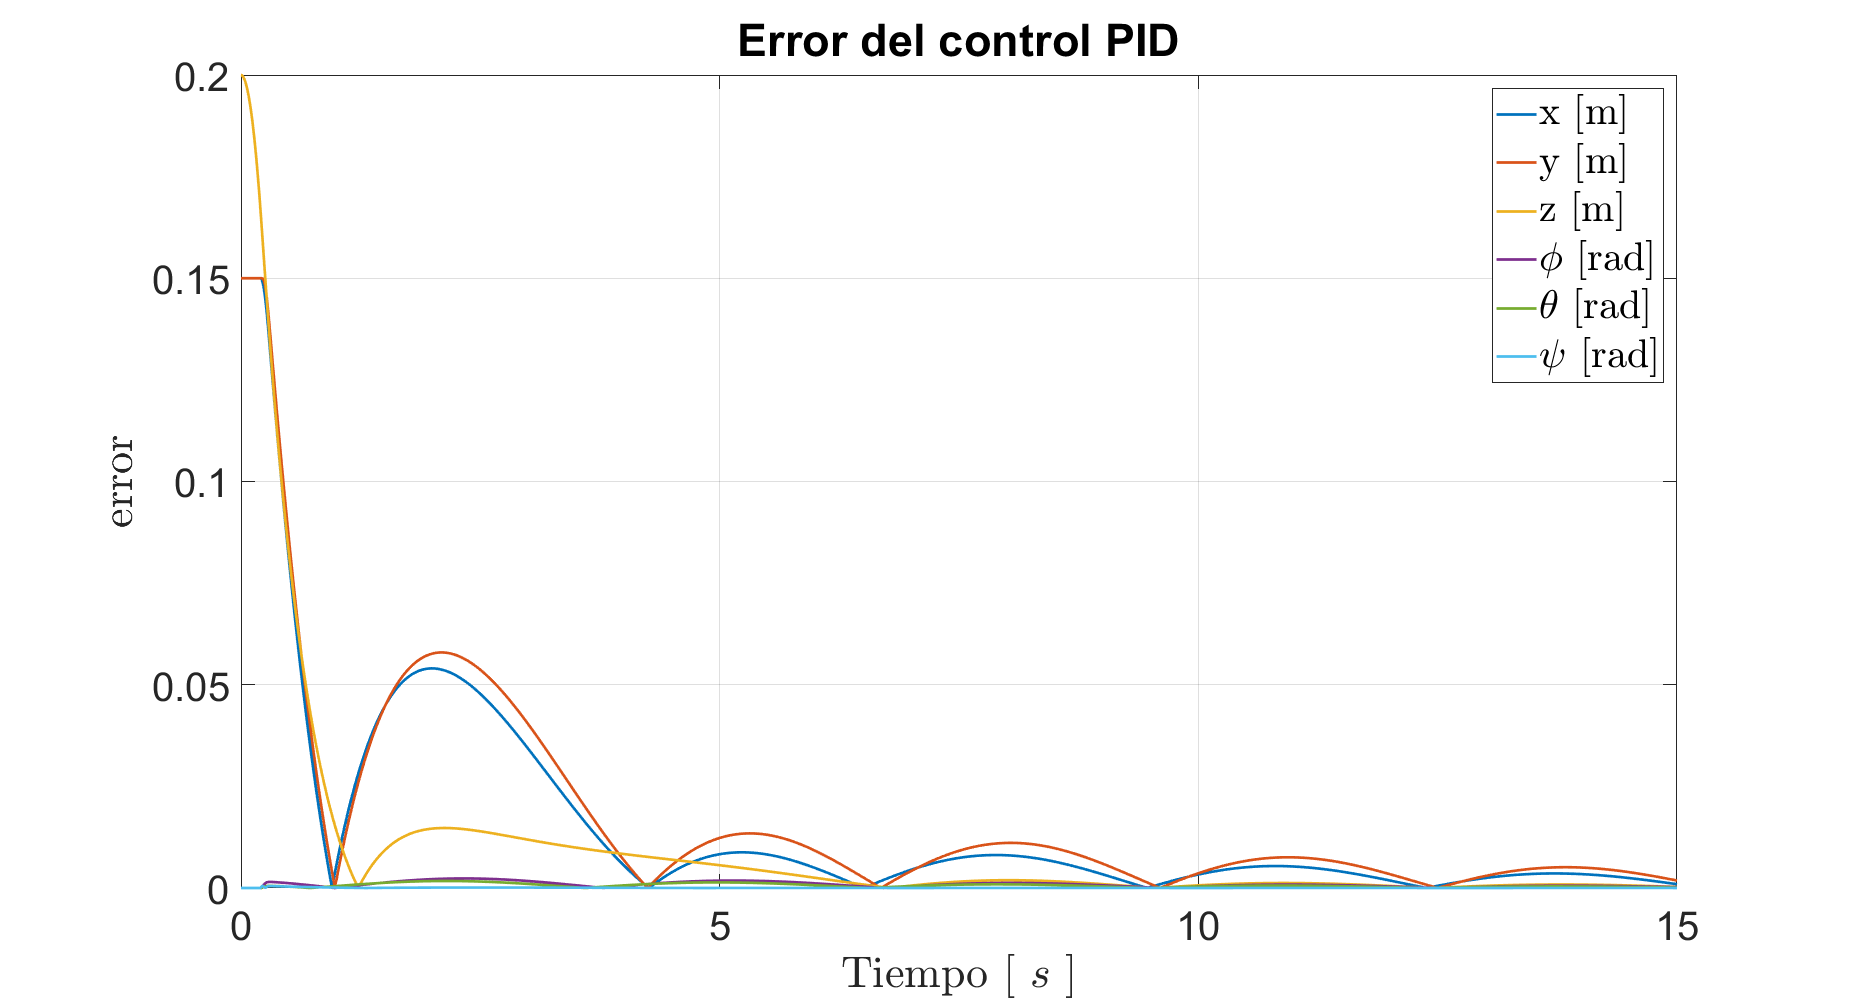
\includegraphics[width=0.4\textwidth]{errorPIDe.png}
    \caption{Error del sistema bajo una referencia estática - PID.}
    \label{fig:PID errore}
\end{figure}

En las figuras \ref{fig:PID position} y \ref{fig:PID error} se observa el comportamiento de la plataforma bajo control PID en la trayectoria generada por las ecuaciones \ref{equ: pos_tray} y \ref{equ: vel_tray}; y a diferencia de los controles anteriores (PD y PD + G) el control PID debido al efecto de la integración se puede eliminar el error ene stado estable. La figura \ref{fig:PID error} muestra como el error durante el movimiento esta constantemente acercandose a cero.

En las figuras \ref{fig:PID positione} y \ref{fig:PID errore} se observa el comportamiento de la plataformas bajo control PID en una referencia estática. Se observa como al igual que en el caso de seguimiento del patron de movimiento se reduce el error en estado estable. Sin embargo aun conserva un pequeño error el cual si se extiende el tiempo de simulación se verá eliminado.

\subsection{Trabajo}

\begin{figure}[H]
    \centering
    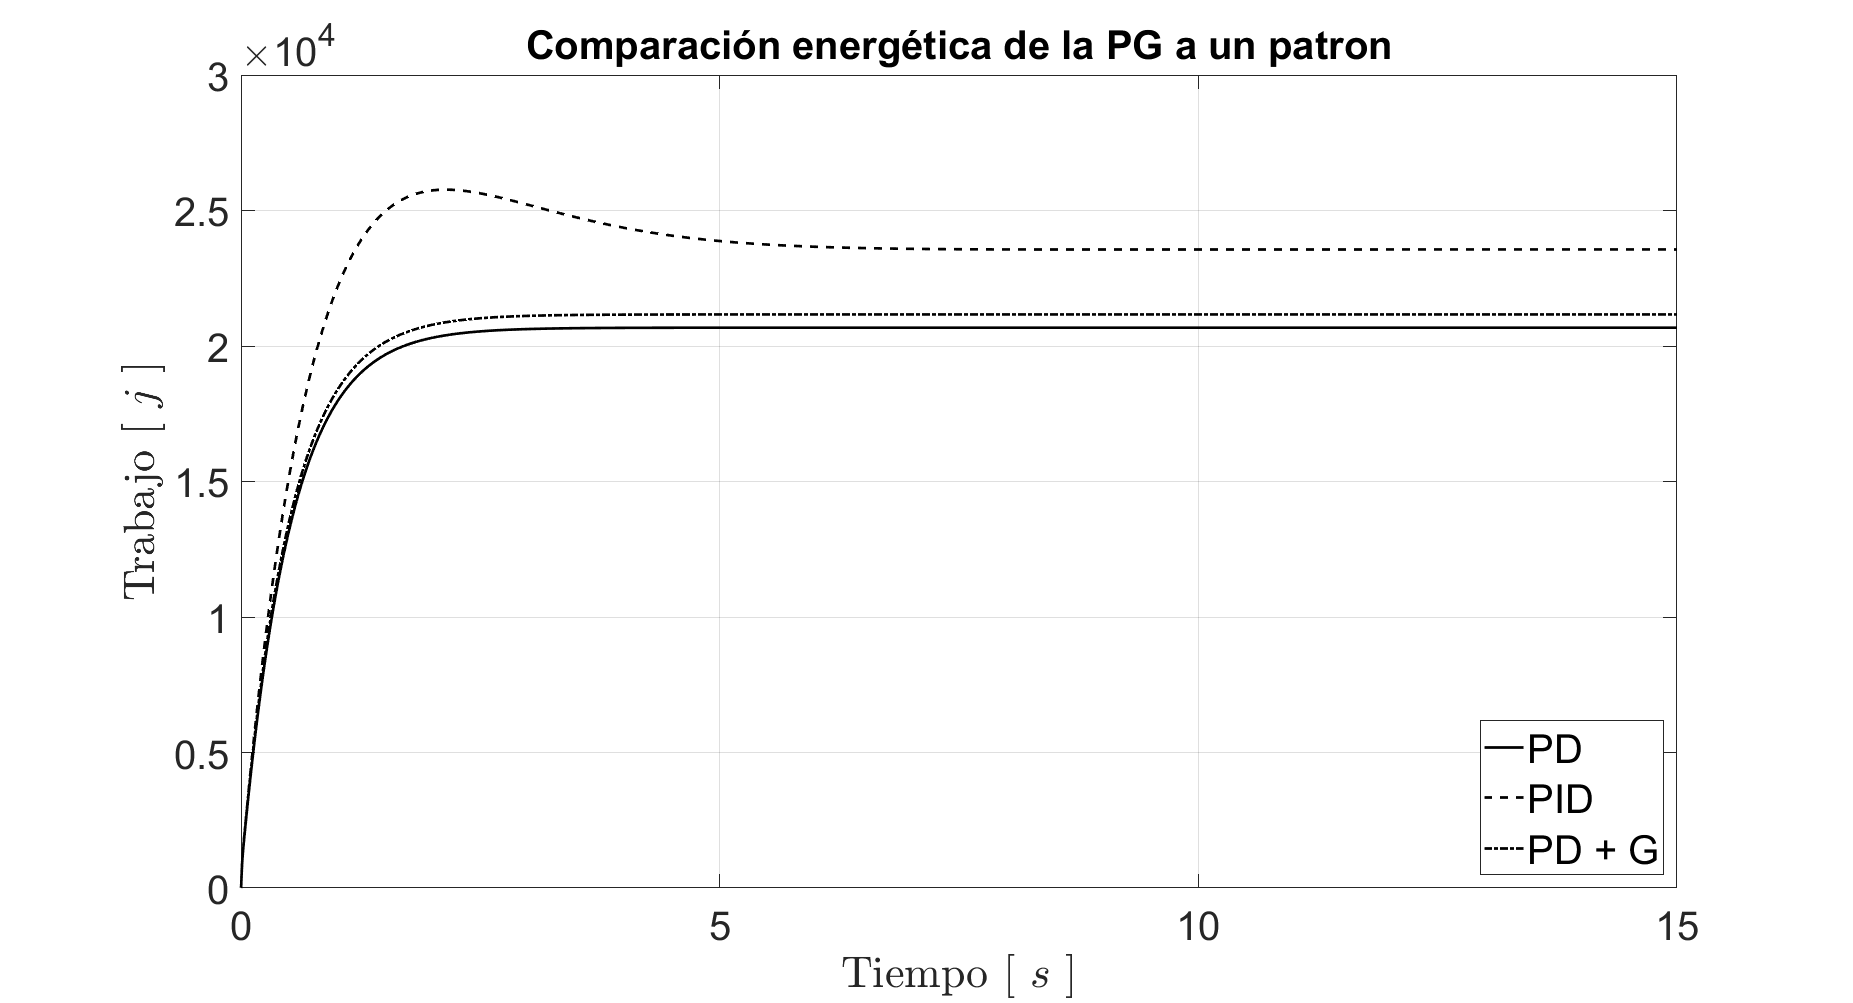
\includegraphics[width=0.4\textwidth]{energiamov.png}
    \caption{Comparación de energía en los diferente controles bajo un patrón de movimiento}
    \label{fig:energiamov}
\end{figure}

\begin{figure}[H]
    \centering
    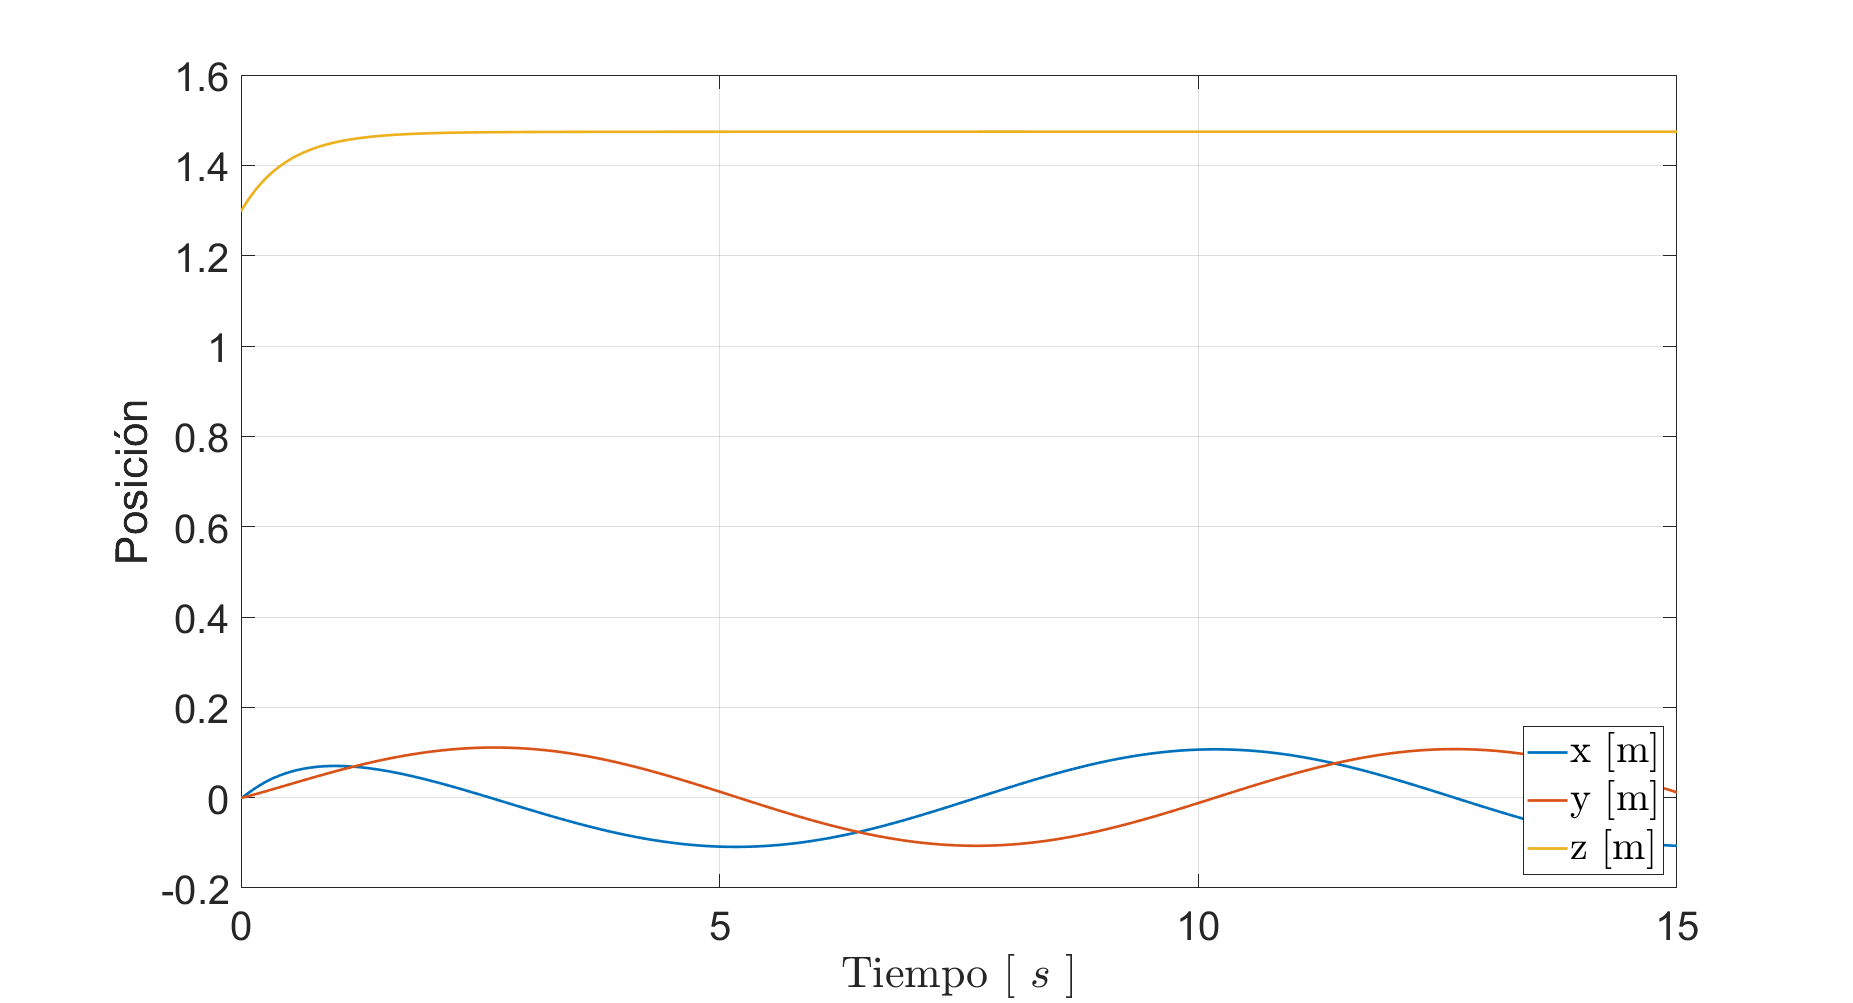
\includegraphics[width=0.4\textwidth]{Energiaestatica.png}
    \caption{Comparación de energía en los diferente controles bajo referencia constante}
    \label{fig:energiaest}
\end{figure}

En las figuras \ref{fig:energiamov} y \ref{fig:energiaest} 